\section{Ogólne określenie wymagań}		%1
%Ogólne określenie wymagań i zakresu programu (Czyli zleceniodawca określa wymagania programu) 

\hspace{0.60cm}Nowoczesne smartfony są naszpikowane różnego rodzaju czujnikami. To one sprawiają, że codzienne używanie telefonów komórkowych jest łatwe i przyjemne. Dzięki nim urządzenia zawsze wiedzą gdzie jesteśmy, w którym kierunku się poruszamy oraz w jaki sposób je trzymamy. Wygaszanie ekranu, gdy zbliżymy słuchawkę do policzka, automatyczna zmiana orientacji wyświetlanego obrazu, kiedy obrócimy telefon czy w końcu sterowanie zaawansowanymi grami - to wszystko nie byłoby możliwe bez czujników. Ogólnym zamysłem naszego projektu jest stworzenie aplikacji która ma służyć do testowania czujników w telefonach, co ułatwiłoby i przyśpieszyło pracę w serwisie komórkowym. Zależy nam na możliwości sprawdzenia czujników takich jak: 
- latarka, \newline 
- test dźwięku, \newline
- bluetooth, \newline
- gps, \newline
- tryb ciemny \newline
- czujnik zbliżeniowy.\newline

Nasza firma powstała w roku 2011; ponad 10 lat prężnie pracujemy oraz staramy się dbać nie tylko o naszych klientów lecz i o naszych pracowników, stąd też pojawił się pomysł na wdrożenie nowej aplikacji, która to pozwoliła by na jeszcze większe usprawnienie pracy w naszym zespole. Co roku zatrudniamy kilkaset nowych osób i to właśnie do nich w dużej mierze miałaby trafić nowa aplikacja. Poprzednie aplikacje, które posiada nasza firma zdecydowanie nie nadają się już do użytku, ponieważ mają wiele mankamentów, takich jak na przykład: brak możliwości wykonania testu GPS'a, który to obecnie jest jednym z najpopularniejszych czujników w telefonach, z którego na co dzień korzysta setki tysięcy osób. Co więcej poprzednie aplikacje miały tendencje do ścinania się tuż po uruchomieniu, dlatego bardzo zależy nam na tym, aby aplikacja funkcjonowała w sposób szybki. Ponadto chcielibyśmy aby aplikacja była zachowana w sposób minimalistyczny i intuicyjny, przez co nawet starsze osoby, które będą z niej korzystać, w szybki sposób będą mogły bez pomocy innych, sprawdzić poszczególne czujniki. Przejrzysta oraz prosta budowa menu, usprawni szukanie odpowiednich komponentów. Mile widziane byłoby zastosowanie panelu logowania w którym to możliwe było by logowanie się do aplikacji poprzez podanie loginu bądź też e-maila oraz hasła. Dzięki temu każdy z naszych pracowników poprzez swój własne dane mógłby w każdej chwili i w każdym miejscu zalogować się do aplikacji.\newline


Kolorem przewodnim naszej firmy jest niebieski, dlatego zależy nam na tym aby akcenty właśnie w tym kolorze pojawiły się w aplikacji; mogą to być na przykład przyciski czy chociażby kolor tła aplikacji. Nasza firma posiada również własne logo, które powinno zawierać się w projekcie.\newline
Na rysunku 1.1 przedstawione jest logo firmy: \newline
%rysunek
\begin{figure}[!hbt]
	\begin{center}
		
\includegraphics[angle=360, width=0.80\textwidth]{rys/logo_black.png}
		\caption{Logo firmy TTest}
		\label{rys:logo}
	\end{center}
\end{figure}
\newline

 Jak wspomnieliśmy powyżej chcielibyśmy również aby pojawił się panel logowania, dzięki któremu zarówno pracownicy jak i klienci będą mogli się zalogować do aplikacji i korzystać z niej bez obaw, że ktoś inny będzie mógł na przykład namierzyć ich lokalizację. Rysunek 1.2 ukazuję przykładowy panel logowania. \newline

\begin{figure}[!hbt]
	\begin{center}
		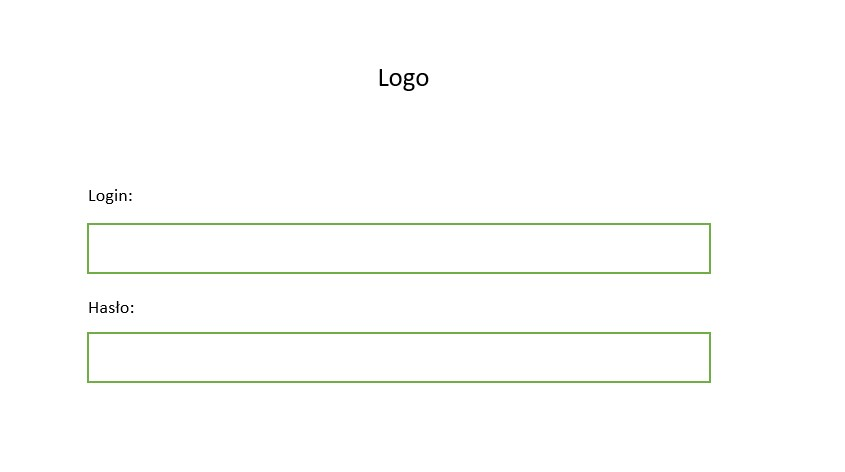
\includegraphics[angle=360, width=0.80\textwidth]{rys/Layout_2.jpg}
		\caption{Przykładowy panel logowania }
		\label{rys:Login}
	\end{center}
\end{figure}
\newpage
 Poniżej na rysunku 1.3 przedstawiamy wstępny layout aplikacji na jakim nam zależy, jeżeli chodzi o przyciski to zależałoby nam na tym aby zamiast wpisanych nazwy tak jak zostało to zaprojektowane na wstępnym layoucie pojawiły się ikonki przedstawiające daną funkcje; na przykład zamiast napisu "Latarka", pojawi się przycisk z wizerunkiem przedstawiającym latarkę; sprawi to że aplikacja będzie wyglądać jeszcze bardziej przejrzyście. \newline
 
 \begin{figure}[!hbt]
 	\begin{center}
 		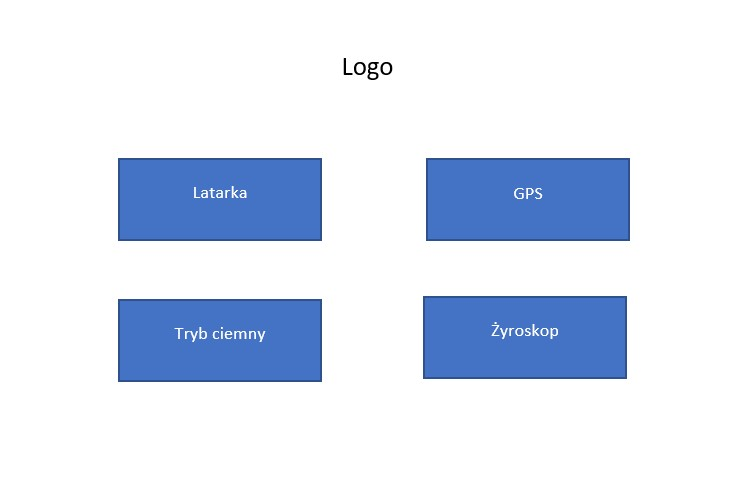
\includegraphics[angle=360, width=0.80\textwidth]{rys/Layout_1.jpg}
 		\caption{Przykładowy layout}
 		\label{rys:Layout}
 	\end{center}
 \end{figure}


  


 
 
 
 
 